%Her beskrives kort hvilken metode der skal anvendes for at løse opgavens tekniske del, f.eks. hvilken analyse- og designmetode, der anvendes. Læseren skal gives et overblik over de anvendte metoder, f.eks. SysML eller UML, med relevante referencer til yderligere litteratur om emnet. Her er det også vigtigt at beskrive eventuelle afvigelser fra teorien i anvendelsen af de metoder I har valgt at benytte. Her beskrives yderligere kort (1-2 sider) den gennemførte proces, set ud fra et interpersonelt synspunkt, dvs. den ikke-tekniske, ”bløde” del af projektet. Dvs. her beskrives overordnede emner som: gruppedannelse, anvendelse af samarbejdsaftaler, arbejdsfordeling, planlægning, møder, projektledelse, projektadministration, iterationer i projektet (iterationer er ”sprints”, hvis der anvendes Scrum). Den gennemførte proces beskrives nærmere i procesbeskrivelsen i projektets bilag.
\newpage
\chapter{Method}
In the following sections the methods used to design and implement the system are described.

\section{ASE-modellen}

The ASE development model structure is shown in figure~\ref{fig:ASE_model}. This has been used to decide what and when to produce in the development process, and has been used in projects in earlier semesters. 

\begin{figure}[H]
	\centering
	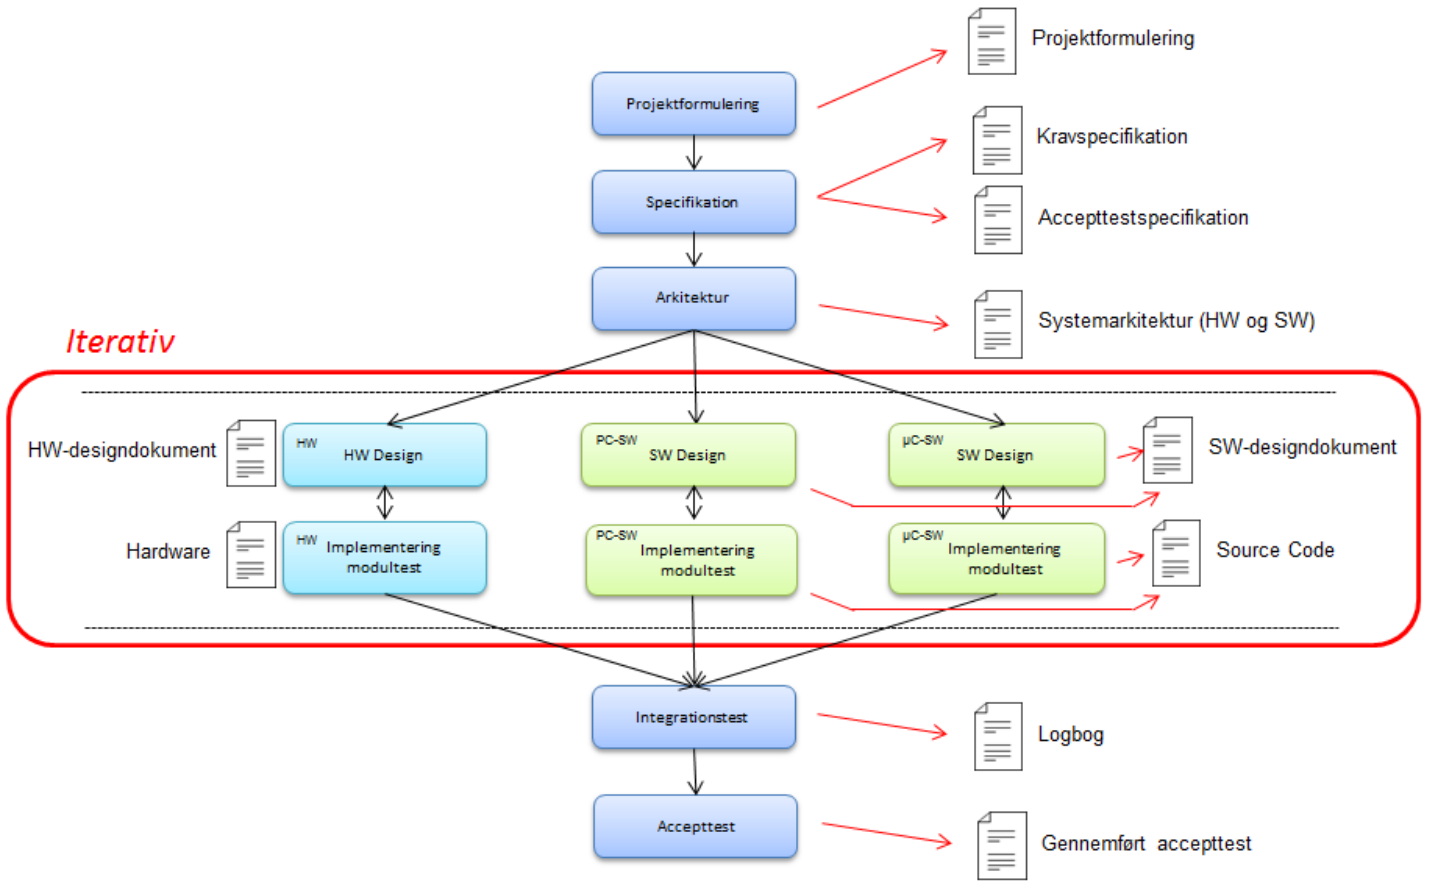
\includegraphics[max width=1\linewidth]{ASE_model.png}
	\caption{ASE development model\cite{ASE_model}}
	\label{fig:ASE_model}
\end{figure}

The model is similar to the waterfall model, where all requirements are specified at the beginning of the project, architecture is developed, and the project enters the design phase. After iterating through design and verification in module tests until all design has been completed, the project undergoes several integration tests, and finally the acceptance test. The test section describes this process in detail.

\section{V-modellen}
The V model in figure ~\ref{fig:V_model} is used for hardware as well as software development, and it describes each development phase and their corresponding test artifacts. 

\begin{figure}[H]
	\centering
	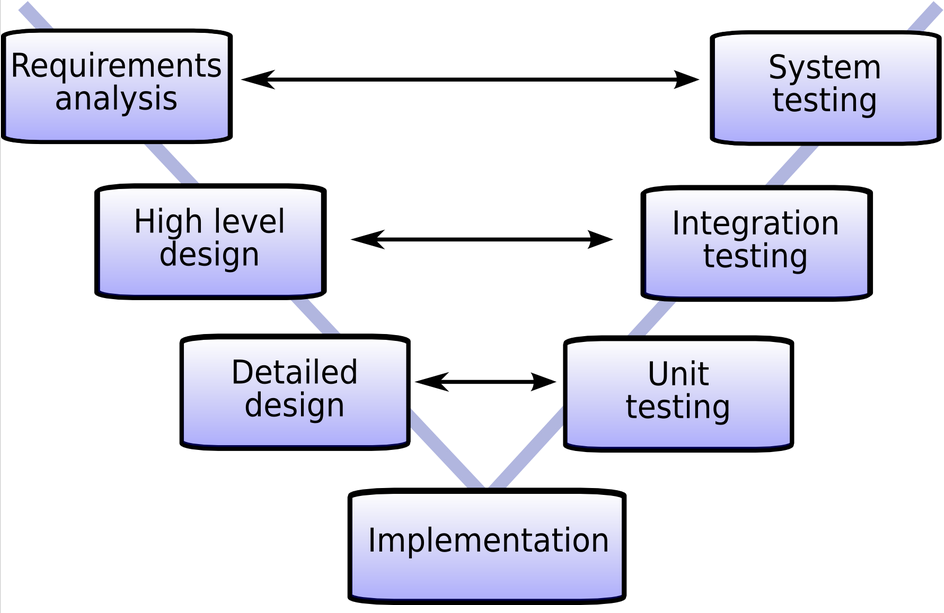
\includegraphics[max width=0.7\linewidth]{V_model.png}
	\caption{The V model}
	\label{fig:V_model}
\end{figure}

The model shows that an acceptance test is specified from the requirements specification, several integration tests are defined from the design, and that the functionality of each module in the system is verified with unit tests. This model is very effective in breaking down the project into several phases and getting an overview of which test phase corresponds to which development phase. The group made extensive use of this approach during development, more about tests can be found in the test section of this document.

\section{SysML}

In developing the architecture and design of the system, SysML has been used as in previous projects. SysML is a way of modeling systems with software and hardware components, where UML, another modeling language, primarily describes software systems. Figure ~\ref{fig:SysML} below gives an overview of the different diagram types in SysML used to describe functionality and design.

\begin{figure}[H]
	\centering
	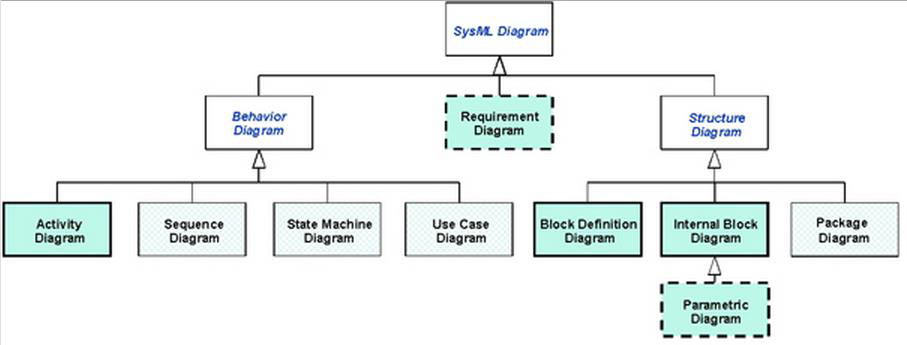
\includegraphics[max width=1\linewidth]{SysML.png}
	\caption{SysML overview\cite{SysML}}
	\label{fig:SysML}
\end{figure}

SysML is widely used in the engineering industry, and enables other developers to quickly gain insight into the system without prior knowledge. 

It is effective in bringing the system from idea to requirements specification, to architecture, and in bridging the gap between architecture and implementation, since SysML describes each module of the system and the logical relation between modules precisely. This also gives clues as to how to to implement the system, particularly in software, since class diagrams can be translated almost directly to internally consistent class hierarchies, if specified in enough detail.

The two structure diagrams used in this system is the Internal Block Diagram (IBD) and the Block Definition Diagram (BDD). The BDD is used to break down the system in its logical blocks, describe the relations between them, and the components of each block. The IBD is used to describe the relationship between the modules primarily in hardware. The IBD typically has a signal list that lists all the signals in the system, their types in the real world, and their values if applicable.

The behavioural diagrams used in this system are the Sequence Diagram (SD) and the Use Case diagram (UC). Use case diagrams describe the actors that interact with the system, and which use cases the system contains. For the software design, an Application Model and Domain Model have been used to describe the behaviour of the software and the overall structure. This is further detailed in the documentation, with class diagrams and function descriptions for each module.

The hardware has been designed from what's called a black-box approach, where the individual components in the IBD are treated as self-contained units. Each component is described in the hardware design section of the documentation.